%
% loesung.tex -- Beispiel-File für die Beschreibung der Loesung
%
% (c) 2020 Prof Dr Andreas Müller, Hochschule Rapperswil
%
\section{Anwendungen
\label{pade:section:Anwendungen}}
\rhead{Anwendungen}

In diesem Kapitel werden ein paar Anwendungsmöglichkeiten für die Verwendung der Padé-Approximation gezeigt.



\subsection{Totzeit Approximation
\label{pade:subsection:totzeit}}

In der Elektrotechnik werden des öfteren mathematische Probleme im Frequenzbereich gelöst da dies oft einfacher ist.
Bei der Totzeit spricht man dabei von einer Verzögerung im Zeitbereich, welcher zum Beispiel in einem Regelkreis vorkommen kann.
Solche Lineare zeitinvariante Systeme (LZI) oder besser bekannt unter dem englischen Begriff linear time-invariant system (LTI), sind unabhängig von zeitlichen Verschiebungen. 
Jeder der sich mit LTI Systemen auseinander gesetzt hat weiss das eine Totzeit $T$ im Bildbereich
\begin{equation*}
H(s) = e^{-sT}
\end{equation*}
durch eine Exponentialfunktion ausgedrückt wird.
Die meisten Übertragungsfunktionen hingegen kommen als gebrochene Polynome, eine Form welche einer rationalen Funktion
\begin{equation*}
H(s)=\frac{P(s)}{Q(s)}
\end{equation*}
entspricht.
Diese gebrochenen Polynome verwendet man dann um Pol- und Nullstellen zu finden um damit dann weitere Analysen durchzuführen. 
Mit $e^{-sT}$ haben wir jedoch keine Polstellen welche wir Analysieren können.
Dies kann jedoch gefordert sein wenn man eine zeit kontinuierliche Analyse machen möchte.
Eine Lösung dafür könnte nun sein $e^{-sT}$ zu approximieren und die Approximation für die weiteren Rechnungen zu verwenden.
Die Padé-Approximation der Exponentialfunktion ist glücklicherweise schon sehr gut bekannt \cite{pade:moler}

\begin{equation}
R_{p, q}(x)
=
\frac{P_{L, M}(x)}{Q_{L, M}(x)} \approx e^{-x}
\end{equation}
wobei $P_{L, M}(x)$ das Zählerpolynom ist
\begin{equation}
P_{L, M}(x)
=
\sum_{j=0}^{L} \frac{(L+M-j) ! L !}{(L+M) ! j !(L-j) !}(-x)^{j}
\end{equation}
und $Q_{L, M}(x)$ das Nennerpolynom der Padéapproximation
\begin{equation}
Q_{L, M}(x)
=
\sum_{j=0}^{M} \frac{(L+M-j) ! M !}{(L+M) ! j !(M-j) !} x^{j}.
\end{equation}
Diesen beide Polynome können verwendet werden um die dazugehörige Padé-Liste 

\begin{equation}\begin{array}{lll}
R_{[1,1]}(x)=\frac{1-\frac{1}{2} x}{1+\frac{1}{2} x} & 
R_{[1,2]}(x)=\frac{1-\frac{1}{3} x}{1+\frac{2}{3} x+\frac{1}{6} x^{2}} & 
R_{[1,3]}(x)=\frac{1-\frac{1}{4} x}{1+\frac{3}{4} x+\frac{1}{4} x^{2}+\frac{1}{24} x^{3}} \\
R_{[2,1]}(x)=\frac{1-\frac{2}{3} x+\frac{1}{6} x^{2}}{1+\frac{1}{3} x} & 
R_{[2,2]}(x)=\frac{1-\frac{1}{2} x+\frac{1}{12} x^{2}}{1+\frac{1}{2} x+\frac{1}{12} x^{2}} &
R_{[2,3]}(x)=\frac{1-\frac{2}{5} x+\frac{1}{20} x^{2}}{1+\frac{3}{5} x+\frac{3}{20} x^{2}+\frac{1}{60} x^{3}} \\
R_{[3,1]}(x)=\frac{1-\frac{3}{4} x+\frac{1}{4} x^{2}-\frac{1}{24} x^{3}}{1+\frac{1}{4} x} &
R_{[3,2]}(x)=\frac{1-\frac{3}{5} x+\frac{3}{20} x^{2}-\frac{1}{60} x^{3}}{1+\frac{2}{5} x+\frac{1}{20} x^{2}} &
R_{[3,3]}(x)=\frac{1-\frac{1}{2} x+\frac{1}{10} x^{2}-\frac{1}{120} x^{3}}{1+\frac{1}{2} x+\frac{1}{10} x^{2}+\frac{1}{120} x^{3}}
\end{array}\end{equation}
zu berechnen.

In der Grafik \ref{pade:totzeitexp} ist ersichtlich das die Approximation mit steigendem Grad bessere Resultate liefert.
Die Grade werden dabei im Nenner und Zähler unterteilt aufgezeigt.
In diesem Beispiel mit der Exponentialfunktion erweisen sich die Polynome des selben Grades im Nenner und Zähler als die geeignetsten.
Wobei mit steigendem Grad eine stetige Verbesserung zugrunde liegt.
\begin{figure}
	\centering
	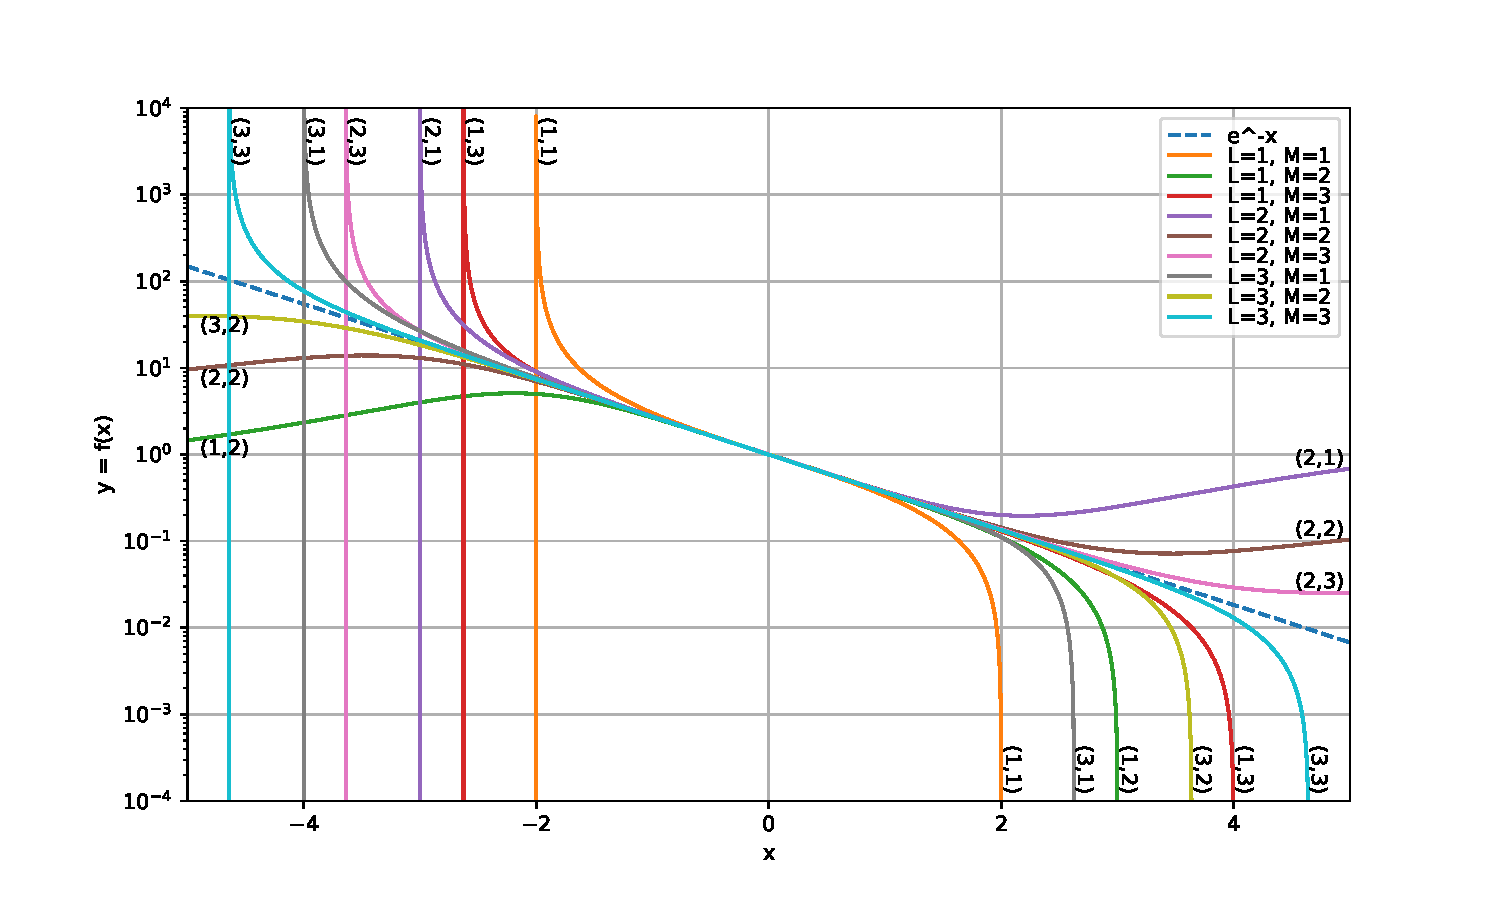
\includegraphics[width=1\linewidth]{./papers/pade/python/bilder/totzeit.pdf}
	\caption{Aufzeigen der Padé-Approximationen der Exponentialfunktion im Vergleich zu der Originalfunktion \label{pade:totzeitexp}}
\end{figure}

Nehmen wir nun diese Polynome und welche noch im Bildbereich sind und transformieren diese wieder zurück in den Zeitbereich erhalten wir die in der Grafik \ref{pade:totzeitexp2} Kurven.
\begin{figure}
	\centering
	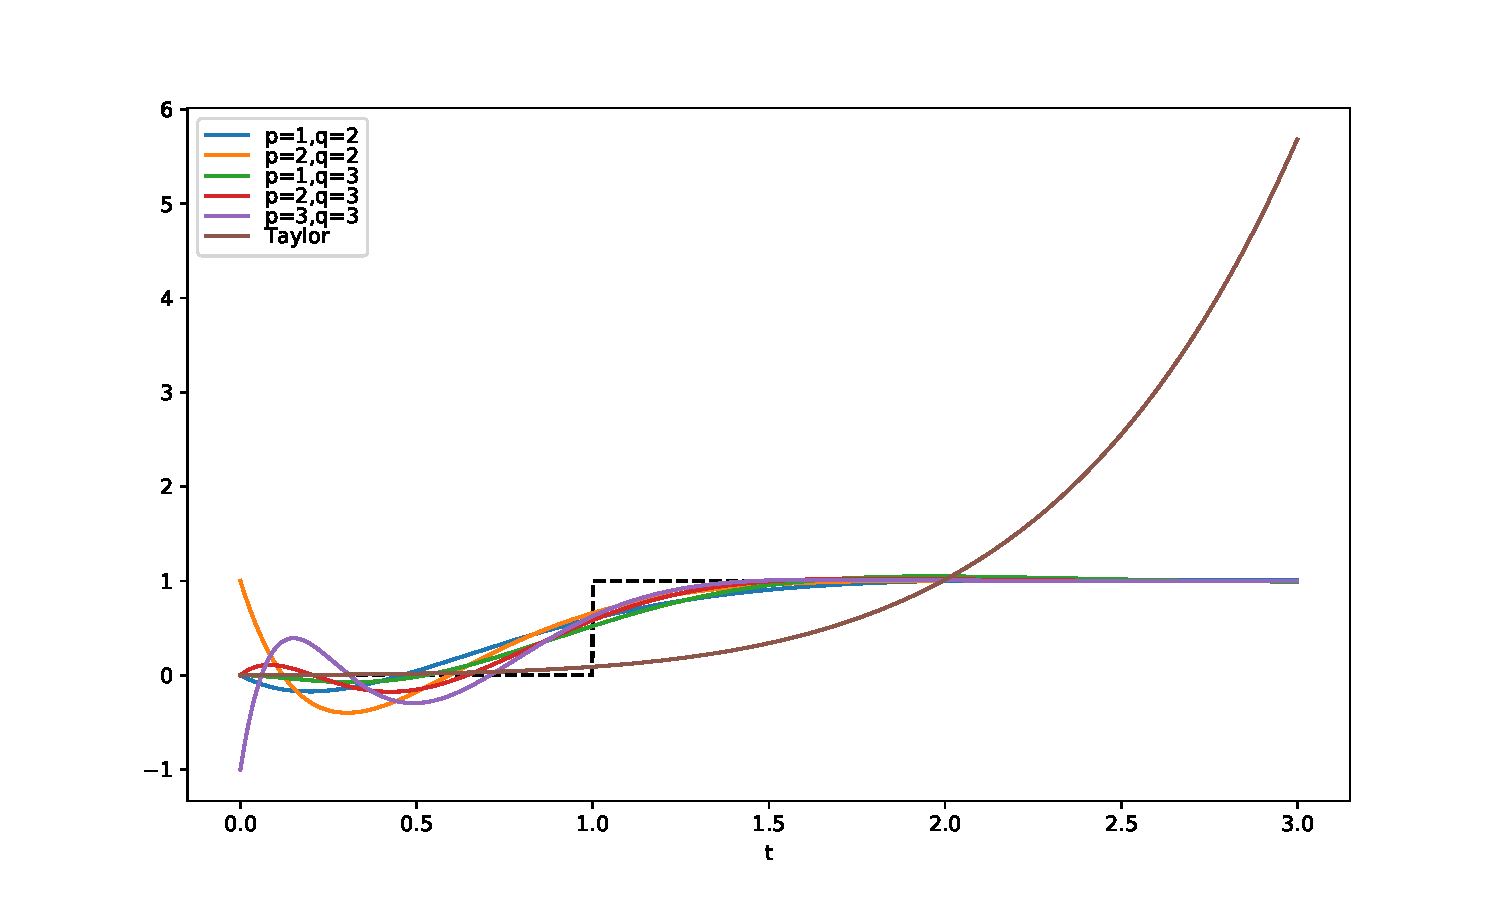
\includegraphics[width=1\linewidth]{./papers/pade/python/bilder/padelow33.pdf}
	\caption{In den Zeitbereich zurück transformierte Polynome \label{pade:totzeitexp2}}
\end{figure}

Die Polynome unterer Ordnung sind dabei noch weit von einem brauchbaren Ergebnis entfernt.

Wenn 












